\chapter{Introduction}

\section{Like Astronomy, but Closer}

Space physics is a field of study that encompasses natural phenomena that occur in our own solar system. The basic difference between it, and the much older field of Astronomy is that in-situ measurements and direct experiments are possible. As a separate field of study, space physics began in earnest at the beginning of the space age with the flights of the first instrumented spacecraft. The discovery of the radiation belts that surround Earth was a profound example of the subsequently rapid increase in knowledge about the space surrounding Earth which is a trend that has continued to the present day. At the same time, and equally importantly, ground based and remote sensing techniques have advanced to the degree that robust, distributed, measurements of the properties of the space around Earth are readily available. The synthesis of these two orthogonal, but complimentary, sources of data gives the field of space physics a distinct image among the sciences, and motivates its pursuit not just for its own sake, but as a window to the workings of the wider universe which we cannot reach.

The space surrounding the Earth is full of activity. To get a picture of this, one can look at the Aurora Borealis, one of the dramatic and beautiful properties of this system. When they occur, the aurora aren't static features. Depending on the type of aurora, they can present as shimmering curtains, pulsing patches, or diffuse regions. These types are not exclusive. Dynamic structures like these, in space and time, are often indicative of a complex system. The old description - that the aurora are caused by the solar wind following the magnetic field of the Earth and hitting the atmosphere - falls flat in light of this complexity. In fact, the current state of knowledge paints a much different picture, with internal properties of the space and constituents surrounding Earth doing most of the ``work'' producing the aurora, which then carries much information about the entire system. 

There are two basic entities in near Earth space: fields and particles, which may be electrically charged. Classical electromagnetism provides a sufficiently accurate description of these in most cases. These are Maxwell's equations, in one of their most common forms:

  \begin{subequations}
    \begin{alignat}{2}
      \mathllap{\text{Gauss' Law}\qquad} && \nabla\cdot\mathbf{E} &= \frac{\rho}{\varepsilon_0} \\
      \mathllap{\text{Gauss' Law ($\mathbf{B}$ Fields)}\qquad} && \nabla\cdot\mathbf{B}  &= 0 \\
      \mathllap{\text{Faraday's Law}\qquad} && \nabla\times\mathbf{E} &= -\frac{\partial \mathbf{B}}{\partial t} \\
      \mathllap{\text{Ampere's Law}\qquad} && \nabla\times\mathbf{B} &= \mu_0\mathbf{J}+\mu_0\varepsilon_0\frac{\partial\mathbf{E}}{\partial t}
      \end{alignat}
        \end{subequations}

In these equations, $\mathbf{E}$ and $\mathbf{B}$ are the electric and magnetic fields, $\mathbf{J}$ is electrical current, $\rho$ is charge density, and $\mu_0 and \varepsilon_0$ are constants. These have been known for a long time, but they contain the root of why the space around Earth is a complicated place. When you have charged particles, they move according to electromagnetic fields, but while they move, they also affect the fields themselves. In an environment like near Earth space, where matter mostly exists as a plasma of charged particles, this gives rise to collective, or self-consistent behaviour and is a source of complexity. Further, a simple analysis of Maxwell's equations shows that wave phenomena also occur. This is combined with the fluid character that particles in large numbers display to make what is called plasma physics. 

Most of the matter in the space around Earth exists as a plasma. Plasma can be roughly defined as a gas of positive and negatively charged particles in approximately equal number, free to move, and at a high temperature. There is a more precise definition, which comes from statistical mechanics. In general, it is accurate to say that one of the defining characteristics of a plasma is the combination of the long-range electromagnetic wave interactions, with short-range collisional and fluid properties. Plasma waves, collective motion, and the propagation, absorption, and emission of radio waves are all observed in the space surrounding Earth. Based on all of this, the overall picture is not one of cold, dark, and empty space, but of a lively and energetic environment, constantly in motion and full of vibrations, with energy, matter, and information constantly flowing.

\begin{figure}[h]
\label{aurora_from_space}
\begin{centering}
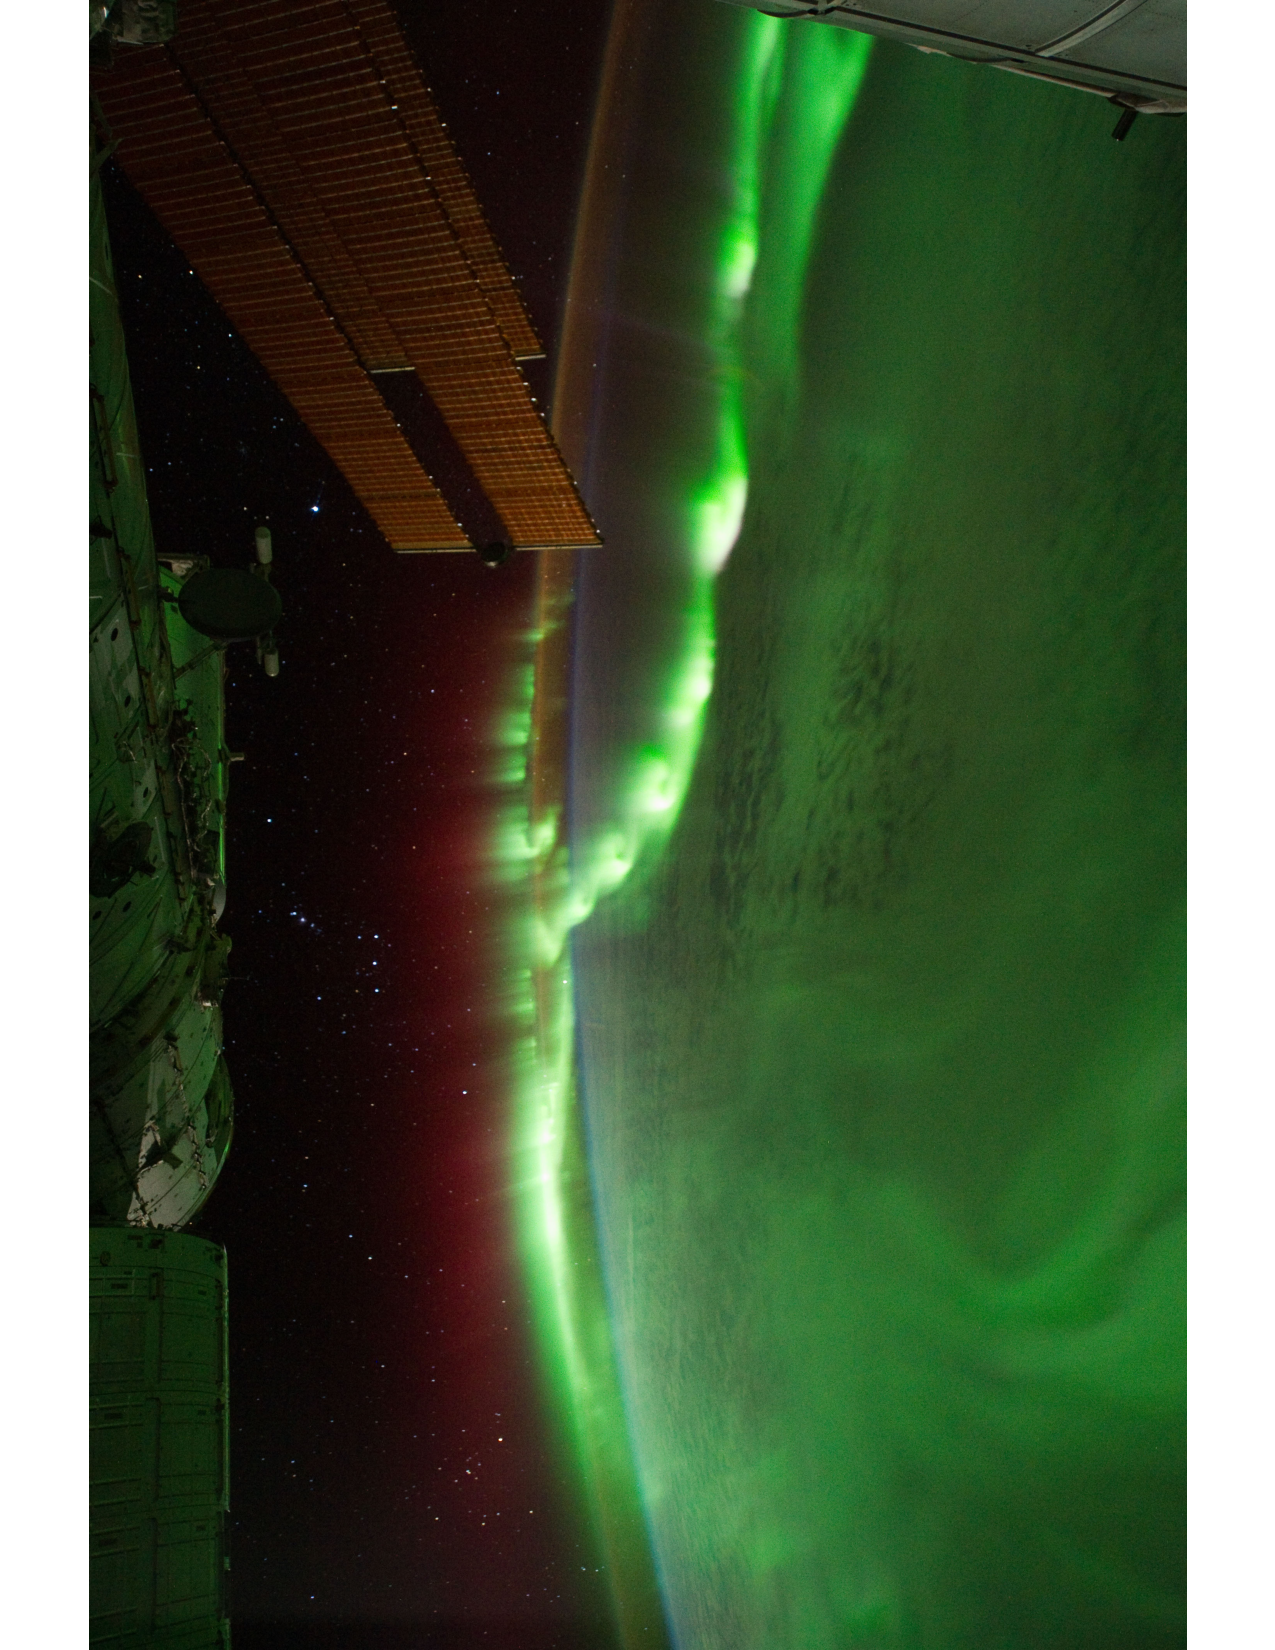
\includegraphics[width=.5\textwidth,angle=270]{figures/chapter_1/aurora_from_space/aurora_from_space}
\caption{This picture of the Aurora, taken from the International Space Station, shows that the space around Earth can have a lively and energetic character. Image by NASA, from nasa.gov.}
\end{centering}
\end{figure}

The active transport of particles through the space around Earth motivates questions about their dynamics. One of the most basic questions is how constituent particles enter and leave the system. Understanding this is central to forming an accurate picture of the overall system. Experimental measurements are required to achieve this. The fact that the Aurora occur is evidence that some fraction of the particles in near-Earth space eventually end up in the atmosphere, where they deposit energy and create visible light. The fact that we can directly observe this secondary radiation makes it a compelling target for experimental measurements. The question then becomes what information about the original particles can be extracted from their impact on the atmosphere. This type of question is not uncommon in the physical sciences. An analogous problem in geophysics is the reconstruction of seismic events  from the vibrations caused at the surface of the Earth. This type of inverse problem naturally leads to a mismatch between the amount of data available and the amount required to generate unique solutions. In this thesis we address the problem of determining the population of electrons leaving geospace by impacting the atmosphere, using measurements of the secondary radiation they produce. Rather than visible light, the secondary X-rays produced by the electrons decelerating in the atmosphere are used as the source of data. 

The aim of this thesis is to develop the techniques necessary to obtain useful information from this indirect measurement. The combination of practical problems due to the need to obtain measurements at high altitudes of greater than 30 kilometers or so, and the mathematical problem of reconstructing useful models from incomplete secondary data lead to a challenging experiment. We show that a surprising amount of detail about the particles in geospace can be found despite these challenges.

\section{The Earth's Atmosphere and Geospace}

The experiments described in this thesis are conducted within the Earth's upper atmosphere, with detectors carried onboard stratospheric balloons. The processes that these experiments measure occur on the boundary between space and the atmosphere.  An accurate description of this region is therefore needed to analyze data from the experiments. 

At the surface of the Earth, the atmospheric constituents are well-mixed. Most of the mass of the atmosphere lies in the region defined as the troposphere, which extends from ground level to to an altitude of around 10 kilometers. This dense region of the atmosphere is where life on Earth, and most terrestrial weather happens. The main structure of the troposphere is defined by a decrease in temperature and density with increasing height. Density decreases exponentially with altitude, which can be shown from the hydrostatic condition. Temperature is somewhat more complicated. Besides local effects (weather), temperature decreasing with height owing to the decreased gravitational potential. The lapse rate defines the rate at which temperature drops with height, and has a value of approximately $2^{\circ}$  C per kilometer of altitude. 

At the tropopause, the temperature of the atmosphere begins to increase with height. The density here is low enough that ultraviolet radiation penetrates and causes the disassociation of molecular oxygen, which results in free oxygen atoms combining with diatomic oxygen to form ozone. The stratosphere is characterized by limited vertical mixing, and is very dry, with few weather effects from the troposphere reaching it. Winds in the stratosphere can be intense, reaching speeds of hundreds of 200 kilometers per hour. This presents interesting operational challenges to experiments carried on balloons in this region, particularly with regards to their post-flight recovery. 

The density in the stratosphere is low, ranging from a few percent of that at ground level to nearly zero at the vertical limit. The low density in the stratosphere makes it quite transparent to certain kinds of radiation from space. In particular, X-rays, created from the slowing down of charged particles farther up in the atmosphere, can propagate deeply in this region. This is where remote sensing of space effects based on secondary radiation becomes possible using balloon-borne instruments, which are discussed in the following section. 

At the end of the stratosphere, temperature once again begins to decrease with height. This occurs at an altitude of approximately 50 kilometers above the surface of the Earth. The mesosphere is the name given to this region of the atmosphere. Here, the different components of the atmosphere are still well-mixed owing to turbulence. This continues to be true to a height of around 80 kilometers. Meteorites burn up in this part of the atmosphere, and the temperature reaches a lower limit of approximately -100 degrees C at its highest point. Once the turbulent effects which occur in the mesosphere become less important, separation of the different atmospheric constituents occurs due to the different scales at which their densities decrease. The hydrostatic condition imposes exponential decreases in density with height, but the scale at which this happens depends on the particle mass. This gives rise to a structure in the upper atmosphere, with the proportions of the different components changes with height. This is important for modelling the propagation of  radiation, which has interactions which depend on the chemical composition, overall density, and temperature. 

Past the mesosphere lies a region called the thermosphere. In this region, temperatures climb sharply and then are steady with increasing height. Solar activity has a strong bearing on the temperatures in this region, which can reach hundreds or thousands of degrees C. Turbulant mixing no longer has meaning at the low densities in the thermosphere. The international definition of the beginning of space, a boundary that begins at 100 kilometers altitude, is contained in this region. In the thermosphere, the density begins to become sufficiently low that the rate of collisions between individual atoms and molecules becomes small enough to start treating them individually, rather than as a fluid. This is the domain where plasmas can exist, since ionized particles and electrons do not immediately collide and become neutral once they are created. This region of space overlaps with the ionosphere, for this reason.  Spacecraft orbit in the thermosphere; orbits with a practical decay time begin at heights of around 350 kilometers.

At heights of hundreds of kilometers, charged particles survive for long enough that electromagnetic interactions become important. Temperature takes on a different intuitive meaning, one based more on the statistical properties of individual and group particle motion, then the classical value that can be measured with a thermometer. The local magnetic field becomes the most important geometry and coordinate system, rather than the local vertical direction from Earth. Free from the dominating effect of collisions, particles undergo characteristic motions not seen in the lower regions of the atmosphere, which are determined by electric and magnetic fields. Figure~\ref{atmosphere_schematic} shows an illustration of some the different layers of the atmosphere, and how the population of charged particles changes with height.

It's not easy to draw a clear sharp line where the atmosphere ends. Such a definition probably needs to depend on the application or line of inquiry being pursued. For aircraft, heights past the stratosphere are unreachable owing to low density. Rockets can reach the intermediate heights between the stratosphere and the thermosphere, while orbiting satellites require further heights still, so that orbits decay on a sufficiently large timescale. Eventually, even the magnetic field of the Earth becomes less important than the magnetic field carried with the plasma of the solar wind, and farther past this point, the influence of the Earth and its magnetic field ceases. The exploration of the solar system, and beyond, by robotic spacecraft begins to  blur the distinction between space physics and astronomy. It is interesting, that the two fields are separated mostly by a practical limitation due to the vast distances involved, instead of a more fundamental, and natural boundary.


\begin{figure}[p]
\label{}
\begin{centering}
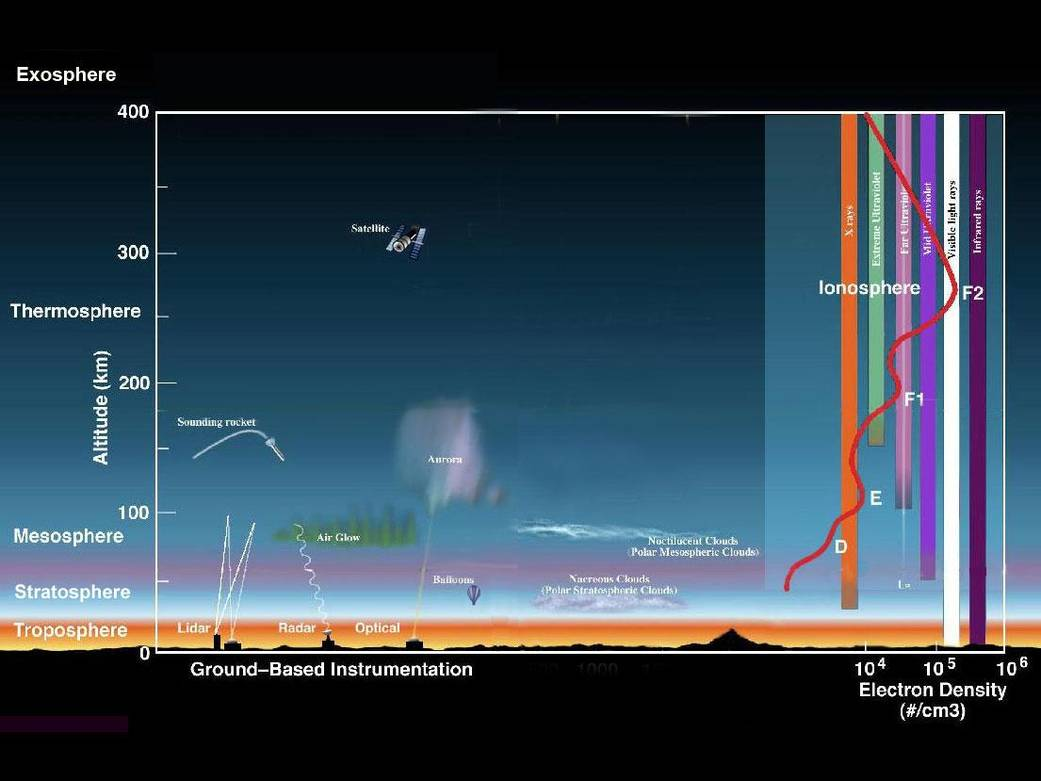
\includegraphics[width=.9\textwidth]{figures/chapter_1/atmosphere_schematic/atmosphere_schematic}
\caption{Schematic illustration showing the scale and structure of the atmosphere, with the overall trend in electron density with height. Image by NASA Goddard, from nasa.gov.}
\end{centering}
\end{figure}
\newpage

\section{Getting Above the Atmosphere with High Altitude Balloons}

Since the atmosphere shields most of the radiation from space, it is not possible to build ground-based experiments that are sensitive to X-ray and charged particle radiation. Rocket flights routinely reach heights where this is no longer a problem, but by their nature, the flight times are short, on the scale of minutes. Orbiting satellites are practical at altitudes far above where radiation from space deposits most of its energy, so there needs to be another kind of vehicle, to get instruments above most of the atmosphere by mass, and that can remain there for hours, or days. Balloons provide data which are distinct from satellites. In the types of balloon experiment conducted in this thesis, radiation detectors are designed with a field of view that extends above them and covers a circle in the sky. The detectors measure secondary radiation produced by energetic particles which enter the atmosphere. On the other hand, satellites do measurements along the path of their orbit, and see particles that have not entered the atmosphere. Additionally, balloons move slowly compared to satellites, and can therefore accomplish measurements of roughly the same region over extended periods.  

Balloons are the vehicles used in this thesis to get above the shielding effects of the lower atmosphere, and measure radiation from space directly at an altitude of 30 to 40 kilometers. High altitude balloons are large, thin, membrane structures, filled with either hydrogen or helium, which carry payloads ranging from grams to hundreds of kilograms, and ascend until they reach an equillibrium height in the stratosphere, above most of the radiation shielding effects of the atmosphere. Balloons need no external energy source to maintain their flight, and so can remain at altitude for hours, days, or even weeks depending on their design and the desired mission profile. With the exception of the balloons needed to carry the largest, heaviest, experiments, high altitude balloons are also inexpensive, compared with rocket flights and satellites. This opens possibilities for extensive surveys and coincident missions which do not exist when using other platforms. 

High altitude balloons follow two distinct designs. The zero-pressure balloon is  named because it maintains an internal pressure equal to the surrounding atmosphere. This is the type of balloon most frequently used for scientific experiments, because it has the property of passively remaining at peak altitude for extended periods of time. The design consists of a large polyethelyne bubble, with one or two vent ducts near the bottom, which are open to the atmosphere. The payload hangs beneath the balloon on a cable or rope. As the balloon is filled through the ducts, lift gas collects at the apex and causes hydrostatic lift. Once a predetermined amount of lift gas has been added, the balloon is released, and ascends, carrying the payload with it. As the balloon ascends, the internal lift gas expands to fill the balloon volume. Eventually, the balloon is completely filled with the low density lift gas, and excess is passively released through the vent ducts, causing the balloon to stop ascending and maintain a fixed altitude. When the balloon mission is terminated, cable cutting equipment is used to separate the payload from the balloon. The payload descends under parachute and is usually recovered. Upon release of the payload, it is typical that the payload rips a destruct panel from the balloon, causing it to release most of its lift gas and descend as well. The point at which the termination process happens is chosen in the design phase of the mission, and can be activated by timer, remote command, or both. 

There is an ultimate limit to the flight duration which can be achieved using zero-pressure balloons, which is caused by internal temperature differences at day and night. During the day, solar radiation warms the balloon and the gas contained in it. When night occurs, the balloon begins to cool, which causes the gas inside to decrease in volume. The balloon has no rigid structure to maintain a fixed volume, so the balloon membrane then occupies less volume as well. This causes the balloon to start to descend, where it reaches a new equillibrium point. At sunrise, solar heating causes the balloon to rise again, although it will not reach the same altitude it started with. For long duration scientific experiments, this  cycle is controlled  through the release of ballast, usually sand. It can be shown that the ultimate limit for the duration of zero pressure balloon flights is approximately 7 days, even if most of the payload consists of expendable ballast. The exception to this rule occurs for flights in the polar regions of the Earth, where the day night cycle is longer. Figure~\ref{zero_pressure_balloon_example} shows a zero-pressure balloon in flight, with the scientific payload being carried below.

\begin{figure}[p]
\label{zero_pressure_balloon_example}
\begin{centering}
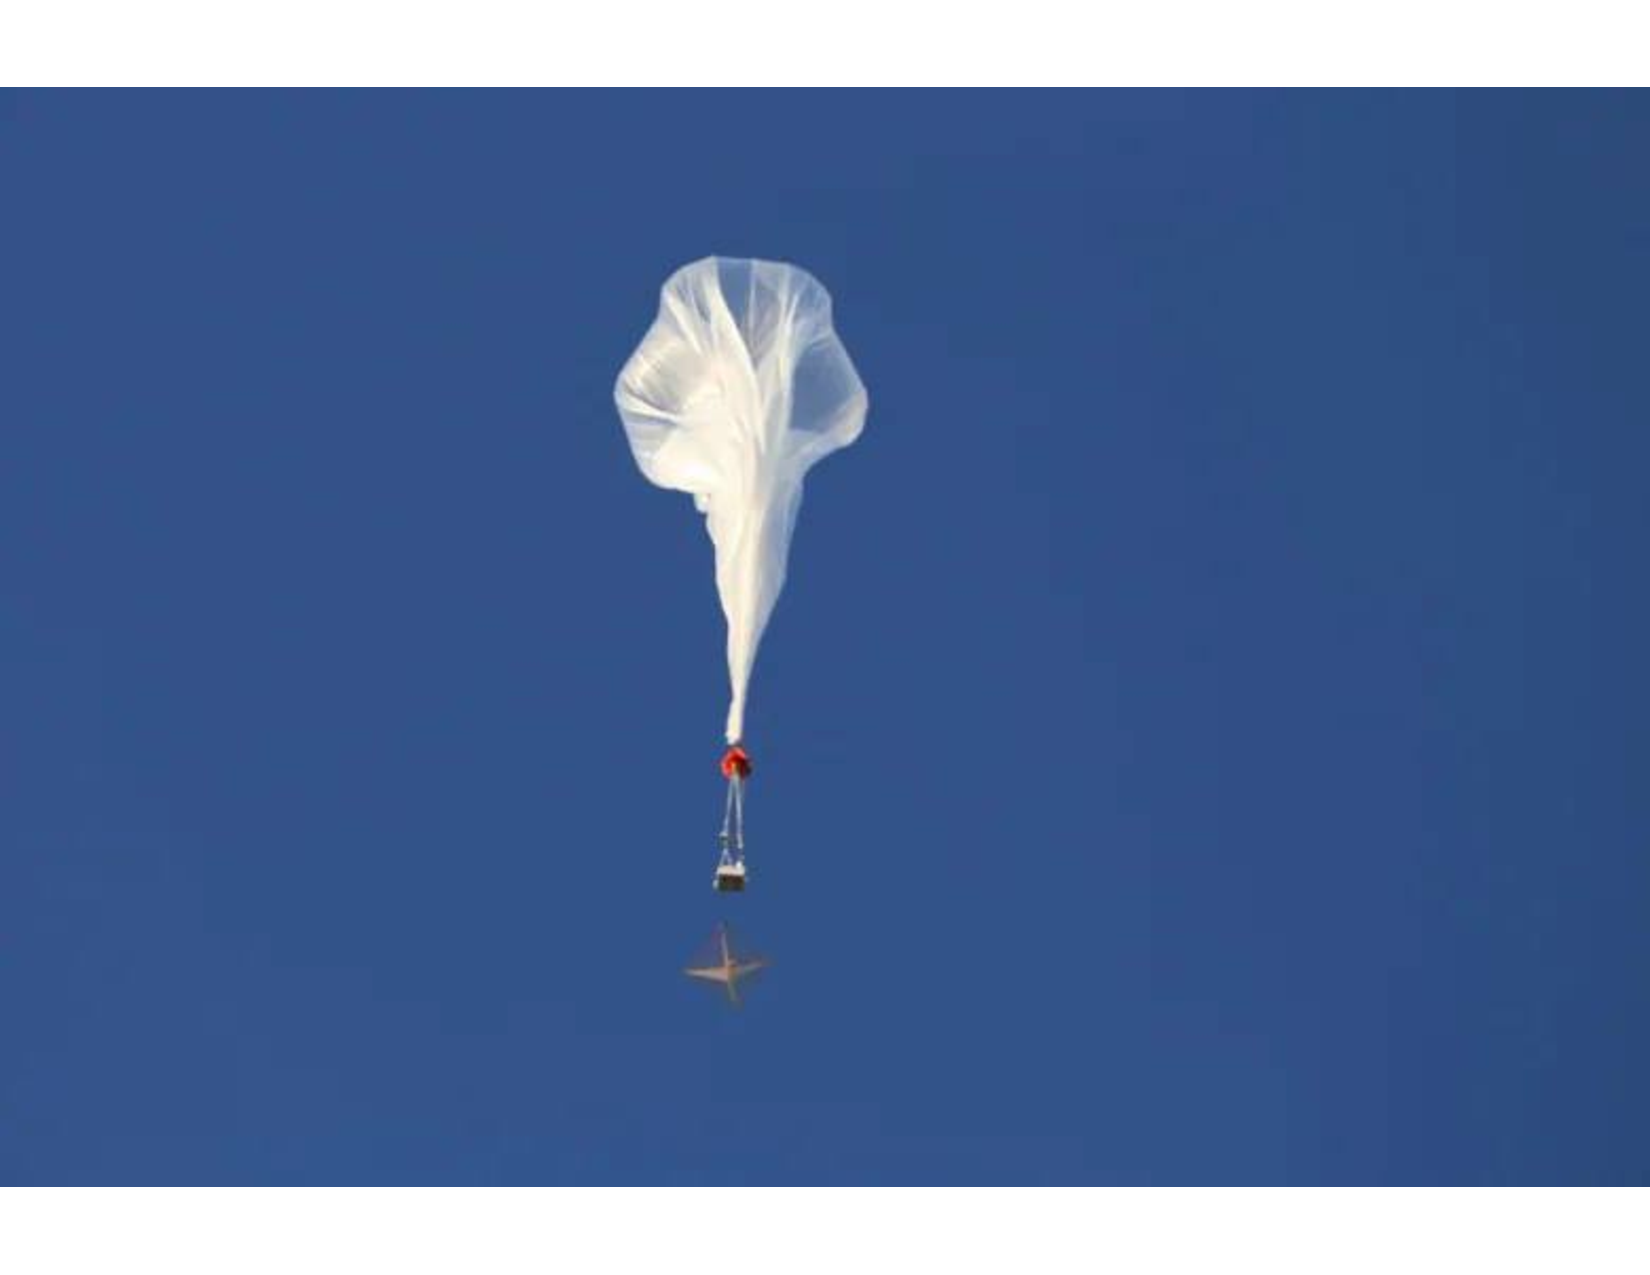
\includegraphics[width=.7\textwidth,angle=270]{figures/chapter_1/zero_pressure_example/zero_pressure_example}
\caption{Zero-pressure balloon in flight shortly after release. The lift gas will expand to fill the balloon volume during the ascent.}
\end{centering}
\end{figure}
\newpage

The second type of high altitude balloon is primarily used for meteorological experiments. Consisting of a relatively small latex sphere, this balloon is closed from the atmosphere and rises until the internal pressure causes it to rupture and descend. These meteorological balloons are launched regularly around the world several times per day to aid in the creation of weather models and forecasts. Typically carrying payloads of only a few hundreds of grams, to at most a few kilograms, these balloons reach heights comparable to the zero-pressure balloons, but do not maintain equillibrium altitude. This makes them less useful for the measurement of space radiation, although, some exotic ways to overcome this problem have been developed and tested.


\section{Scope of this Thesis}

The question is: what is the maximum amount of information that can be obtained about processes far out in the space surrounding Earth, using measurements of the resulting radiation, and what kinds of instruments do we need to use to get the requisite data? This question is interesting because the experiments take place on the boundary between what we can directly affect using active experiments, and what we only learn through passive observation. Right now, most experimentalists are earth-bound, and this is unlikely to change in the near future. On the other hand, the types of experiments we fly on high altitude balloons provide a window to the wider universe, in a way that, unlike orbiting spacecraft, which require years or decades of planning, can be rapidly iterated on and repeated. The upper atmosphere can be thought of as a giant laboratory, and a detector which is sensitive to the radiation incident upon it from space. We have the ability to send experiments to this region rapidly and at low comparative cost to spacecraft. There is therefore a scientific return on being able to maximize the information we obtain from these experiments. The problem of mapping the available measurements of secondary radiation back to the particles impacting the atmosphere is required for this to happen. The following chapters will show the development of a solution which can be used to increase the observational power of balloon-borne experiments.

 


